\documentclass[11pt]{article}
\ifdefined\pdfinfoomitdate\pdfinfoomitdate=1\fi
\ifdefined\pdftrailerid\pdftrailerid{}\fi
\ifdefined\pdfsuppressptexinfo\pdfsuppressptexinfo=15\fi
\usepackage[T1]{fontenc}
\usepackage{lmodern}
\usepackage[margin=1.05in]{geometry}
\usepackage{amsmath,amssymb,amsthm,mathtools}
\usepackage{microtype,needspace}
\usepackage{tikz}
\usetikzlibrary{arrows.meta,patterns}
\usepackage{xurl}
\usepackage[colorlinks=true,linkcolor=blue!45!black,citecolor=blue!45!black,urlcolor=blue!45!black]{hyperref}
\hypersetup{pdftitle={Edit Distance in l1: Matching Bounds up to Constants in the Exponent},pdfauthor={OpenAI}}
\urlstyle{same}
\newcommand{\ED}{\operatorname{ED}}
\newcommand{\ID}{\Delta}
\newcommand{\LCS}{\operatorname{LCS}}
\newcommand{\ellone}{\ell_1}
\newcommand{\E}{\mathbb E}
\newcommand{\R}{\mathbb R}
\newcommand{\Z}{\mathbb Z}
\newcommand{\eps}{\varepsilon}
\newcommand{\enc}{\operatorname{enc}}
\newcommand{\norm}[1]{\left\lVert#1\right\rVert_1}
\newtheorem{theorem}{Theorem}[section]
\newtheorem{proposition}[theorem]{Proposition}
\newtheorem{lemma}[theorem]{Lemma}
\newtheorem{corollary}[theorem]{Corollary}
\theoremstyle{remark}
\newtheorem{remark}[theorem]{Remark}
\numberwithin{equation}{section}
\setlength{\emergencystretch}{2em}
\allowdisplaybreaks[1]
\title{Edit Distance in \texorpdfstring{$\ell_1$}{l1}:\\
Matching Bounds up to Constants in the Exponent}
\author{OpenAI}
\date{September 27, 2026}
\begin{document}
\maketitle
\begin{abstract}
We determine the exponential scale of the least $\ell_1$ distortion of
unit-cost edit distance on all strings of length at most $d$. For every
sufficiently large $d$, uniformly over finite alphabets of size at least
two, the distortion lies between
$\exp(c\sqrt{\log d\,\log\log d})$ and
$\exp(C\sqrt{\log d\,\log\log d})$ for absolute constants $c,C>0$.
The lower bound already holds on binary strings of one common length.
Thus the order of logarithmic distortion is sharp up to absolute constants.
\end{abstract}

\section{Introduction}

We study how faithfully distances between strings can be represented by
distances in $\ell_1$. The distance on strings is ordinary edit distance:
$\ED(x,y)$ is the least number of single-symbol insertions, deletions and
substitutions that transform $x$ into $y$, with every operation costing
one. An insertion or deletion changes the positions of an entire suffix.
As a result, the distance depends on the best alignment of the two strings,
and a useful representation must account for alignments over all scales.

For a finite alphabet $\Sigma$ and an integer $d\ge1$, let
$\Sigma^{\le d}$ be the set of all strings of length at most $d$, including
the empty string. The cap restricts the endpoints; intermediate strings
in an edit script may have any length. Write $\ell_1$ for the real space of
absolutely summable sequences and define
\[
 E_\Sigma(d)=
 \inf_{f:\Sigma^{\le d}\hookrightarrow\ell_1}
 \left(\max_{x\ne y}\frac{\norm{f(x)-f(y)}}{\ED(x,y)}\right)
 \left(\max_{x\ne y}\frac{\ED(x,y)}{\norm{f(x)-f(y)}}\right).
\]
The infimum is over injective maps. It imposes no restriction on target
dimension or on the cost of computing the map. Equivalently, an embedding
has distortion at most $D$ when it can be rescaled so that every image
distance lies between $\ED(x,y)/D$ and $\ED(x,y)$.

\Needspace{11\baselineskip}
\begin{theorem}\label{thm:main}
There are absolute constants $c,C>0$ and an integer $d_0$ such that, for
every integer $d\ge d_0$ and every finite alphabet $\Sigma$ with
$|\Sigma|\ge2$,
\begin{equation}\label{eq:main}
 \exp\!\bigl(c\sqrt{\log d\,\log\log d}\bigr)
 \le E_\Sigma(d)\le
 \exp\!\bigl(C\sqrt{\log d\,\log\log d}\bigr).
\end{equation}
The lower bound is witnessed by a subset of binary strings of one common
length at most $d$. The same bounds hold for
$\sup_{\Sigma:\,2\le|\Sigma|<\infty}E_\Sigma(d)$.
\end{theorem}

Logarithms are natural unless a base is specified. The constants and
threshold in the theorem are independent of the alphabet, including when
its size grows with $d$. The conclusion determines the order of
$\log E_\Sigma(d)$; the constants in the exponent remain unspecified.

\subsection*{The earlier bounds}

The single-symbol error model is classical. Levenshtein studied codes
correcting insertions, deletions and substitutions
\cite{Levenshtein1966}, and Wagner and Fischer described edit scripts
through increasing traces \cite{WagnerFischer1974}. Their alignment
language will be useful below: any lower bound must control every
increasing matching of equal symbols, including matchings that cross the
boundaries used to construct the strings.

Ostrovsky and Rabani \cite{OstrovskyRabani2007} proved the upper scale in
Theorem~\ref{thm:main} for fixed-length binary strings by recursively
comparing collections of overlapping substrings. They also noted
extensions to larger alphabets and varying lengths. We use their
fixed-length theorem and give complete reductions with constants uniform
over all finite alphabets and with the empty string included.

For lower bounds, Andoni, Deza, Gupta, Indyk and Raskhodnikova
\cite{AndoniDezaGuptaIndykRaskhodnikova2003} constructed binary subsets
whose $L_1$ distortion approaches $3/2$. Khot and Naor
\cite[Theorem~4.1]{KhotNaor2006} obtained an
$\Omega(\sqrt{\log d/\log\log d})$ lower bound by
studying cuts and Fourier analysis of noisy shifts. Their
insertion--deletion metric is within a factor of two of the convention
used here. Krauthgamer and Rabani
\cite[Theorem~1.3]{KrauthgamerRabani2009} then proved an
$\Omega(\log d)$ lower bound for binary strings of length $d$.
The construction below reaches the scale of the Ostrovsky--Rabani
exponent.

\subsection*{How the lower bound works}

The construction joins a geometric fact about strings to an analytic
fact about $\ell_1$. At the geometric level, a word is a long list of
rows. Each row contains a payload made of lower-level words, followed by
a long marker consisting of a fresh symbol. The payload has fixed slots;
each slot has its own alphabet tag, so different slots cannot match.
The lower-level words depend on states. In each component, repeatedly
adding one distinguished step cycles the state with a prime period;
different components use different primes.
Advancing every component by one state step shifts the row list by one,
which costs only the deletion and insertion of one row.

Advancing the distinguished component behaves differently. We repeat
that component in many separately tagged slots. For any proposed pair
of rows, either those repeated slots remain separated or the row shift
that aligns them leaves many of the other prime-period components
separated. A global alignment can still send one source payload into
several target rows. In that event, the matching skips a complete target
marker: the source payload contains no copy of the marker symbol.
The skipped markers for different payloads are disjoint. This turns
the row comparison into a lower bound for arbitrary alignments.

The analytic comparison concerns the average image distance produced
by a group displacement. Proposition~\ref{prop:displacement} bounds
the displacement in the distinguished component by the simultaneous
step and the average component steps. The proof expresses a finite
$\ell_1$ metric as a nonnegative sum of cut metrics, then expands each
cut in Fourier characters. A character involving few components is
detected by the simultaneous step: distinct prime denominators prevent
its phase from being an integer. A character involving many components
is detected by the sum of the component averages.

Relative to word length, the guaranteed pointwise separation decreases
by a fixed factor at each level. Under the same normalization, the
analytic inequality forces the allowed averaged image displacement
to decrease much faster: after $k$ levels, the ratio between these two
bounds is $\exp(\Omega(k\log k))$. Meanwhile, the logarithmic word
length is $O(k^2\log k)$. A delimiter code transfers the words to binary
with a loss polynomial in $k$, and choosing $k$ directly from the cap $d$
supplies a witness for every sufficiently large $d$.

Section~\ref{sec:displacement} proves the alignment facts and the
prime-product displacement inequality. Section~\ref{sec:construction}
builds the words and proves their separation and analytic recurrence
together. Section~\ref{sec:binary} supplies the delimiter at the
binary transfer and completes the parameter calculation.
Section~\ref{sec:upper} derives the uniform upper bound by hashing the
alphabet, padding to one binary length, and averaging over all hash maps.

The companion manuscripts on circle constructions \cite{OpenAICircle2026}
and tree constructions \cite{OpenAITree2026} give independent lower-bound
mechanisms and additional binary coding results. No result from a companion
manuscript is used; the upper bound uses the stated external theorem.

\section{Alignments and a displacement inequality}\label{sec:displacement}

The word construction will be measured first by insertion--deletion
distance. Its advantage is that every possible comparison has a concrete
description as an increasing matching. We then state the analytic
inequality that will be applied at each level of the construction.

\subsection{Distances from increasing matchings}

Write $\ID(x,y)$ for the minimum number of single-symbol insertions and
deletions transforming $x$ into $y$. An increasing matching is a list of
pairs of equal-symbol positions, strictly increasing in both coordinates.
Let $\LCS(x,y)$ be its maximum size. These are the classical trace and
subsequence descriptions of string correction
\cite[Sections~3 and~5]{WagnerFischer1974}.

\begin{lemma}\label{lem:alignments}
For arbitrary finite strings, including the empty string,
\begin{equation}\label{eq:metric-comparison}
 \ED(x,y)\le\ID(x,y)\le2\ED(x,y),
 \qquad
 \ID(x,y)=|x|+|y|-2\LCS(x,y).
\end{equation}
For two strings of the same length $n$, define their one-sided deficit by
\[
 r_n(x,y)=n-\LCS(x,y)=\tfrac12\ID(x,y).
\]
A matching of size $n-E$ leaves exactly $E$ unmatched positions on each
side.
\end{lemma}

\begin{proof}
An insertion--deletion script is an edit script, and replacing each
substitution by one deletion and one insertion proves the two
inequalities. Deleting the unmatched source positions in an increasing
matching and inserting the unmatched target positions realizes its
total loss $|x|+|y|-2|M|$. Conversely, the original positions that
survive an insertion--deletion script form an increasing matching; its
loss is at most the number of operations. Minimizing the loss gives the
identity. The equal-length assertions follow directly.
\end{proof}

\subsection{The comparison to be proved}

For a finite abelian group $G$ and a map $H:G\to\ell_1$, set
\begin{equation}\label{eq:variation}
 V_H(g)=\E_{z\in G}\norm{H(z+g)-H(z)}.
\end{equation}
Every expectation over a finite set uses the uniform probability measure.
The following proposition compares a shift in one component with a
simultaneous shift and with shifts averaged inside the separate
components. In the word construction, the simultaneous shift will move
the row list by one; the component averages will be bounded at the
preceding level.

\begin{proposition}[Prime-product displacement inequality]
\label{prop:displacement}\label{fourier:displacement}
Let $b,h\ge1$ be integers, let $P\ge1$, and let $G_1,\ldots,G_b$ be finite
abelian groups. Suppose $v_j\in G_j$ has order $p_j$, where
$p_1,\ldots,p_b$ are distinct primes in $[P,2P]$. In
$G=\prod_{j=1}^bG_j$, use the same notation $v_j$ for the element acting
only in coordinate $j$, and put $\tau=\sum_{j=1}^b v_j$. Then every
$H:G\to\ell_1$ and every integer $u$ satisfy
\begin{equation}\label{eq:prime-product-bound}
 V_H(uv_1)
 \le (2P)^{2h}V_H(\tau)
 +\frac2h\sum_{j=1}^b\E_{a\in\Z/p_j\Z}V_H(av_j).
\end{equation}
\end{proposition}

We prove the proposition after recording two elementary forms of the
cut and Fourier methods. The cut representation is standard
\cite[Section~4]{LinialLondonRabinovich1995}. Its summability statement
below permits an unrestricted sequence-space target.

\begin{lemma}[Finite cut decomposition]\label{lem:cuts}
Let $X$ be finite and $H:X\to\ell_1$. There are finite numbers $c_A\ge0$,
indexed by the nonempty proper subsets of $X$, such that
\begin{equation}\label{eq:cuts}
 \norm{H(x)-H(y)}
 =\sum_{\varnothing\ne A\subsetneq X}
 c_A|\mathbf1_A(x)-\mathbf1_A(y)|
 \qquad(x,y\in X).
\end{equation}
Moreover,
\[
 \sum_{\varnothing\ne A\subsetneq X}c_A
 \le\sum_{\{x,y\}\subset X,\ x\ne y}\norm{H(x)-H(y)},
\]
where the right sum is over unordered pairs.
\end{lemma}

\begin{proof}
For $|X|\le1$ all the sums are empty. Otherwise, for coordinate $n$ of
$H$, list its distinct values on $X$ as
$t_{n,1}<\cdots<t_{n,k_n}$. Put
\[
 A_{n,r}=\{x:H_n(x)>t_{n,r}\},\qquad
 a_{n,r}=t_{n,r+1}-t_{n,r}\quad(1\le r<k_n).
\]
The consecutive gaps telescope:
\[
 |H_n(x)-H_n(y)|
 =\sum_{r=1}^{k_n-1}a_{n,r}
 |\mathbf1_{A_{n,r}}(x)-\mathbf1_{A_{n,r}}(y)|.
\]
Group all terms with the same cut by setting
$c_A=\sum_{n,r:\,A_{n,r}=A}a_{n,r}$, initially allowing the value
$+\infty$. Nonnegativity allows the coordinate series to be interchanged
with the finite sum over unordered pairs. Hence
\[
 \sum_{\varnothing\ne A\subsetneq X}c_A|A|\,|X\setminus A|
 =\sum_{\{x,y\}\subset X,\ x\ne y}\sum_{n=1}^{\infty}
 |H_n(x)-H_n(y)|
 =\sum_{\{x,y\}\subset X,\ x\ne y}\norm{H(x)-H(y)}<\infty.
\]
Each indexed cut separates at least one pair, so
$|A|\,|X\setminus A|\ge1$. The displayed equality proves that all the
weights are finite and bounds their total. Summing the coordinate
identity and grouping its nonnegative terms now gives \eqref{eq:cuts}.
\end{proof}

\begin{lemma}[Finite Fourier displacement identity]\label{lem:fourier}
Let $T=\prod_{j=1}^b\Z/p_j\Z$, where the integers $p_j$ are at least two.
For $\lambda\in T$, set
\[
 \chi_\lambda(t)=
 \exp\!\left(2\pi\mathrm i\sum_{j=1}^b\frac{\lambda_jt_j}{p_j}\right),
 \qquad
 \widehat F(\lambda)=\E_{t\in T}F(t)\overline{\chi_\lambda(t)}.
\]
For every $F:T\to\mathbb C$ and $l\in T$,
\begin{equation}\label{eq:fourier-displacement}
 \E_{t\in T}|F(t+l)-F(t)|^2
 =\sum_{\lambda\in T}|\widehat F(\lambda)|^2
 4\sin^2\!\left(\pi\sum_{j=1}^b\frac{l_j\lambda_j}{p_j}\right).
\end{equation}
The squared sine is independent of the chosen integer representatives.
\end{lemma}

\begin{proof}
The geometric-series identity
\[
 \frac1p\sum_{a=0}^{p-1}e^{2\pi\mathrm iqa/p}
 =\begin{cases}
 1,&p\mid q,\\
 0,&p\nmid q
 \end{cases}
\]
shows, coordinate by coordinate, that the $|T|$ characters are
orthonormal for the inner product
$\langle F_1,F_2\rangle=\E_tF_1(t)\overline{F_2(t)}$.
They form a basis because the function space has dimension $|T|$.
Thus $F(t)=\sum_\lambda\widehat F(\lambda)\chi_\lambda(t)$, and the
squared norm equals the sum of squared Fourier coefficients. Apply this
to
\[
 F(t+l)-F(t)
 =\sum_\lambda\widehat F(\lambda)
       (\chi_\lambda(l)-1)\chi_\lambda(t)
\]
and use $|e^{2\pi\mathrm i\theta}-1|^2=4\sin^2(\pi\theta)$.
\end{proof}

\begin{proof}[Proof of Proposition~\ref{prop:displacement}]
By Lemma~\ref{lem:cuts}, each displacement of $H$ is a nonnegative
linear combination of displacements of Boolean cut maps. It is enough
to prove \eqref{eq:prime-product-bound} for one such map
$H=\mathbf1_A$.

Let $K=\prod_j\langle v_j\rangle\subseteq G$. Every shift in the desired
inequality preserves every coset of $K$. On a fixed coset, choose a
representative $c$ and identify
$T=\prod_j\Z/p_j\Z$ with that coset through
$t\mapsto c+\sum_jt_jv_j$. The cut becomes
$F(t)=\mathbf1_A(c+\sum_jt_jv_j)$. For Boolean values, absolute
difference equals squared difference. With
$D_F(l)=\E_t|F(t+l)-F(t)|^2$, it remains to prove
\begin{equation}\label{eq:coset-bound}
 D_F(ue_1)\le(2P)^{2h}D_F(\mathbf1)
 +\frac2h\sum_{j=1}^b\E_{a\in\Z/p_j\Z}D_F(ae_j),
\end{equation}
where $\mathbf1=(1,\ldots,1)$ and $e_j$ is the $j$th coordinate vector.

We compare the multipliers in Lemma~\ref{lem:fourier} one frequency at
a time. Fix $\lambda\in T$, write
$S=\{j:\lambda_j\ne0\}$ and $r=|S|$. When $\lambda_1=0$, the
left multiplier vanishes. Assume therefore that $\lambda_1\ne0$.
The left multiplier is at most four.

First suppose $r<h$. Choose $0\le\lambda_j<p_j$ and put
\[
 q=\prod_{j\in S}p_j,\qquad
 \theta=\sum_{j\in S}\frac{\lambda_j}{p_j}.
\]
For any $i\in S$, distinctness of the primes gives
$q\theta\equiv\lambda_i(q/p_i)\not\equiv0\pmod{p_i}$.
Thus $\theta$ is not an integer. Since its denominator divides $q$,
its distance $\delta$ from the nearest integer satisfies
\[
 \frac12\ge\delta\ge\frac1q
 \ge(2P)^{-r}\ge(2P)^{-h}.
\]
Concavity of sine on $[0,\pi/2]$ gives
$\sin(\pi\delta)\ge2\delta$. Consequently the simultaneous-shift
multiplier on the right of \eqref{eq:coset-bound} is at least
\[
 (2P)^{2h}4\sin^2(\pi\theta)
 =(2P)^{2h}4\sin^2(\pi\delta)\ge16,
\]
which bounds the left multiplier.

Now suppose $r\ge h$. For each coordinate, the same geometric-series
identity gives
\[
 \E_{a\in\Z/p_j\Z}4\sin^2(\pi a\lambda_j/p_j)
 =2-2\operatorname{Re}\E_a e^{2\pi\mathrm ia\lambda_j/p_j}
 =\begin{cases}2,&j\in S,\\0,&j\notin S.\end{cases}
\]
The component terms on the right therefore have combined multiplier
$(2/h)2r\ge4$, again bounding the left. This case includes $h=1$.
Multiplication by $|\widehat F(\lambda)|^2$ and summation over
$\lambda$ proves \eqref{eq:coset-bound}. Averaging over the equal-size
cosets gives the uniform average over $G$. Finally, summing the
nonnegative cut weights proves the proposition for $H$.
\end{proof}

The two cases explain the role of distinct periods. A low-support
frequency pays for a nonintegral simultaneous phase; a high-support
frequency pays for many component variations. The next section turns
these two payments into an iterated obstruction.

\section{Recursive words with incompatible displacements}
\label{sec:construction}

We now build the words to which Proposition~\ref{prop:displacement}
will be applied. The row list must be long enough that its one-row shift
remains inexpensive after multiplication by $(2P)^{2h}$ in that
inequality. At the same time, it must be shorter than the
product of many component periods, so that a row shift cannot cancel
too many prime-period differences. The following choices provide both
properties.

Fix a sufficiently large integer $k$ and set
\begin{equation}\label{eq:parameters}
 b=100k,\qquad P=b^2,\qquad h=b/10=10k,\qquad L=P^{b/2}.
\end{equation}
Choose $b$ distinct primes in $[P,2P]$, and call their set
$\mathcal P$. The prime number theorem gives
$\pi(2P)-\pi(P)\sim P/\log P>b$ for all sufficiently large $k$;
the explicit interval estimate of Rosser and Schoenfeld
\cite[Corollary~3, equation~(3.8)]{RosserSchoenfeld1962} also gives
this consequence. We use this one pool and the same parameters at
every level.

\subsection{The recursive family and its cheap steps}

For every $0\le s\le k$ and $p\in\mathcal P$, the construction supplies
a finite abelian state group $G_{s,p}$, a distinguished element
$v_{s,p}$ of order $p$, and a word map
\[
 W_{s,p}:G_{s,p}\longrightarrow\mathcal A_{s,p}^{\,n_s}.
\]
It also supplies a finite list $\mathcal S_{s,p}$ of pairs $(e,r)$,
where $e\in G_{s,p}$ is a step and $r>0$ is its displacement budget.
The word map itself need not be injective. Define
\begin{equation}\label{eq:recurrences}
 \alpha_s=24^{-s},\qquad Q_0=2,\qquad
 Q_s=\frac{2(2P)^{2h}}{L}+\frac{Q_{s-1}}h.
\end{equation}

\begin{proposition}[Recursive properties]\label{prop:family}
The families can be chosen with
\[
 n_s=\bigl(2(2b-1)L\bigr)^s,\qquad
 |\mathcal A_{s,p}|\le A_s,\qquad
 A_0=2P,\quad A_s=1+(2b-1)A_{s-1},
\]
so that the following assertions hold.
\begin{enumerate}
\item Every listed step is cheap at every state:
\begin{equation}\label{eq:step-property}
 \ID\bigl(W_{s,p}(z),W_{s,p}(z+e)\bigr)\le n_s r
 \quad\bigl((e,r)\in\mathcal S_{s,p},\ z\in G_{s,p}\bigr).
\end{equation}
\item Every nonzero distinguished shift is separated at every state:
\begin{equation}\label{eq:far-property}
 \ID\bigl(W_{s,p}(z),W_{s,p}(z+uv_{s,p})\bigr)\ge n_s\alpha_s
 \quad(z\in G_{s,p},\ 1\le u<p).
\end{equation}
\item If $H:G_{s,p}\to\ell_1$ satisfies the averaged budgets
$V_H(e)\le r$ for all $(e,r)\in\mathcal S_{s,p}$, then
\begin{equation}\label{eq:l1-property}
 V_H(uv_{s,p})\le Q_s\qquad(1\le u<p).
\end{equation}
\end{enumerate}
\end{proposition}

The first two assertions describe the geometry of the words. The third
says that any $\ell_1$ map respecting the same cheap-step budgets has
small average displacement in the separated direction. We prove the
proposition by simultaneous induction on $s$, constructing the word maps
and the cheap-step lists together.

At level zero, take
\[
 G_{0,p}=\Z/p\Z,\quad v_{0,p}=1,\quad
 W_{0,p}(z)=(z),\quad
 \mathcal S_{0,p}=\{(e,2):e\ne0\}.
\]
The single symbols are distinct. Their insertion--deletion distance is
two, so the first two assertions hold with $n_0=1$ and $\alpha_0=1$.
The listed budgets give the third assertion with $Q_0=2$.
The alphabet has $p\le2P$ symbols.

Suppose the families at level $s-1$ have been constructed. To build
the family indexed by $p$, enumerate the pool as $p_1,\ldots,p_b$ with
$p_1=p$, and abbreviate
\[
 G_j=G_{s-1,p_j},\quad v_j=v_{s-1,p_j},\quad
 W_j=W_{s-1,p_j},\quad m=n_{s-1}.
\]
Set
$G_{s,p}=\prod_{j=1}^bG_j$ and
$v_{s,p}=(v_1,0,\ldots,0)$, which has order $p$.

For $z=(z_1,\ldots,z_b)$, the new word is a concatenation of $L$ rows,
indexed by $i=0,\ldots,L-1$. Row $i$ begins with a payload of $2b-1$
slots. Its first $b$ slots contain separately tagged copies of
$W_1(z_1+iv_1)$; its remaining slots contain tagged copies of
$W_j(z_j+iv_j)$ for $j=2,\ldots,b$, in that order. Each slot has its
own tag, fixed across all rows and different from every other slot tag.
The payload length is
$B=(2b-1)m$. Append a marker $\#^B$, where $\#$ is absent from all
payloads.

More formally, the new alphabet is the disjoint union of $\{\#\}$ and
one set $\{r\}\times\mathcal A_{s-1,p_j}$ for each slot $r$ carrying
component $j$. This also tags every lower-level marker, so none becomes
the new symbol $\#$. The full length and alphabet bounds are
\begin{equation}\label{eq:row-length}
 n_s=2BL=2(2b-1)L\,n_{s-1},
 \qquad |\mathcal A_{s,p}|\le1+(2b-1)A_{s-1}.
\end{equation}

There are two kinds of cheap steps. First include the simultaneous
step $\tau=(v_1,\ldots,v_b)$ with budget $2/L$. Row $i$ of the word at
$z+\tau$ is row $i+1$ of the word at $z$ whenever $0\le i<L-1$.
Deleting the first row and inserting one final row costs at most
$4B=2n_s/L$.

For the other steps, let $c_1=b$ and $c_j=1$ for $j\ge2$, and put
\begin{equation}\label{eq:weights}
 \omega_j=\frac{c_jm}{2B},\qquad \sum_{j=1}^b\omega_j=\frac12.
\end{equation}
The number $\omega_j$ is the fraction of the full word occupied by
component $j$; markers occupy the other half. For each
$(e,r)\in\mathcal S_{s-1,p_j}$ include its lift $\widetilde e$ to
coordinate $j$ with budget $\omega_jr$. The preceding level's bound
holds at every translated state $z_j+iv_j$. Editing the $Lc_j$ affected
slots separately therefore costs at most
$Lc_jmr=n_s\omega_jr$. This proves \eqref{eq:step-property}.

\subsection{Separation across row boundaries}\label{sec:separation}

We first isolate the matching argument supplied by the fresh markers.
It will convert a comparison of every pair of payloads into a comparison
of the full row lists.

\begin{lemma}[Marked payloads]\label{lem:marked}
Let $T,p,q\ge1$ be integers, let $\Gamma$ be an alphabet, and let
$\#\notin\Gamma$. For $U_a,V_b\in\Gamma^p$ with $1\le a,b\le T$, put
\[
 X=U_1\#^q\cdots U_T\#^q,\qquad
 Y=V_1\#^q\cdots V_T\#^q,\qquad N=T(p+q).
\]
If $d\ge0$ and $r_p(U_a,V_b)\ge d$ for every $a,b$, then
\begin{equation}\label{eq:marked}
 r_N(X,Y)\ge\frac{Tdq}{d+q}\ge\frac T2\min(d,q).
\end{equation}
In particular, $d\le q$ implies $\ID(X,Y)\ge Td$.
\end{lemma}

\begin{proof}
Fix an increasing matching, with $E$ unmatched positions on each side.
No source payload symbol can match a target marker. Let $s$ be the
number of source payloads whose matches reach at least two target
payloads.

A source payload whose matches lie in one target payload loses at least
$d$ source positions. A payload with no matches loses $p\ge d$ positions.
Summing over these $T-s$ payloads gives $E\ge d(T-s)$.

For each of the other $s$ payloads, choose a target marker between two
of its matches, as in Figure~\ref{fig:marker}. The entire marker is
unmatched: a matched target
position between the two chosen matches would have its source partner
between their source partners, inside this source payload, where $\#$
does not occur. The target matched spans of different source payloads
are ordered and disjoint, so the chosen markers are distinct. Thus
$E\ge sq$.

Combining the two estimates gives $E\ge d(T-E/q)$ and hence
$E\ge Tdq/(d+q)$. The latter is at least
$(T/2)\min(d,q)$. This holds for every matching, including when $d=0$,
and proves \eqref{eq:marked}. Finally $\ID(X,Y)=2r_N(X,Y)$.
\end{proof}

\begin{figure}[t]
\centering
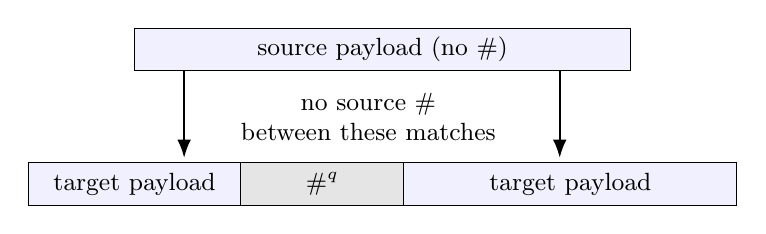
\begin{tikzpicture}[x=0.9cm,y=0.9cm,>=Latex,font=\small]
 \draw[fill=blue!6] (1.5,1.9) rectangle (8.5,2.5);
 \node at (5,2.2) {source payload (no $\#$)};
 \draw[fill=blue!6] (0,0) rectangle (3,0.6);
 \draw[fill=gray!20] (3,0) rectangle (5.3,0.6);
 \draw[fill=blue!6] (5.3,0) rectangle (10,0.6);
 \node at (1.5,0.3) {target payload};
 \node at (4.15,0.3) {$\#^q$};
 \node at (7.65,0.3) {target payload};
 \draw[->,thick] (2.2,1.9)--(2.2,0.67);
 \draw[->,thick] (7.5,1.9)--(7.5,0.67);
 \node[align=center] at (4.8,1.25)
       {no source $\#$\\between these matches};
\end{tikzpicture}
\caption{Two matches from one source payload enclose an unmatched target
marker. The arrows represent matched pairs; no alignment of other payload
boundaries is assumed.}\label{fig:marker}
\end{figure}

We apply the lemma to the words at $z$ and $z+uv_{s,p}$, where
$1\le u<p_1$. Compare source payload $i$ with target payload $i'$ and
write $\delta=i'-i$. Their relative shifts are $(\delta+u)v_1$ in
component $1$ and $\delta v_j$ in component $j\ge2$.

At least $b/3$ slots have a nonzero shift. If $p_1\nmid\delta+u$, all $b$
copies of component $1$ do. Otherwise $\delta\ne0$, since $1\le u<p_1$.
Now $0<|\delta|<L=P^{b/2}$, whereas the product of $b/2$ distinct primes
from the pool is at least $P^{b/2}$. Fewer than $b/2$ pool primes can
therefore divide $\delta$. Among components $2,\ldots,b$, at least
$b-1-b/2\ge b/3$ have a nonzero shift.

In each such slot the induction hypothesis gives
insertion--deletion distance at least $m\alpha_{s-1}$. A matching of
the two complete length-$m$ slot words therefore leaves at least
$m\alpha_{s-1}/2$ source positions unmatched. Since the slot tags are
disjoint, every matching between the two payloads restricts to a
matching of the corresponding complete slot words. Its size is bounded
by their $\LCS$ even if other source payloads use some positions of the
same target slot. Thus every pair of payloads has one-sided deficit at
least
\[
 d_s=\frac{\alpha_{s-1}bm}{6}.
\]
We have $d_s\le B$. Lemma~\ref{lem:marked}, with $T=L$ and marker
length $B$, gives
$\ID(W_{s,p}(z),W_{s,p}(z+uv_{s,p}))\ge Ld_s$. Dividing by
\eqref{eq:row-length},
\[
 \frac{\ID(W_{s,p}(z),W_{s,p}(z+uv_{s,p}))}{n_s}
 \ge\frac{\alpha_{s-1}b}{12(2b-1)}
 \ge\frac{\alpha_{s-1}}{24}=\alpha_s.
\]
This proves the pointwise separation \eqref{eq:far-property}.

\subsection{The averaged analytic recurrence}\label{sec:averaged}

Suppose $H:G_{s,p}\to\ell_1$ meets the listed averaged budgets.
We need the preceding level's assertion for one component, but its
hypotheses concern averages over that component's entire state group.
The right map is a direct sum over all settings of the other components.

For fixed $j$, let $Y_j=\prod_{\ell\ne j}G_\ell$ and define
\begin{equation}\label{eq:slice-map}
 T_j(x)=\frac1{\omega_j|Y_j|}
          \bigoplus_{y\in Y_j}H(x,y),\qquad x\in G_j.
\end{equation}
Here $H(x,y)$ means that $x$ occupies coordinate $j$, and the finite
direct sum of sequence spaces is identified with $\ell_1$. For every
$e\in G_j$, additivity of the sum norm gives
\begin{equation}\label{eq:slice-identity}
 V_{T_j}(e)
 =\frac1{\omega_j}\E_{x\in G_j,\,y\in Y_j}
       \norm{H(x+e,y)-H(x,y)}
 =\frac{V_H(\widetilde e)}{\omega_j}.
\end{equation}
The lifted step budgets therefore make $T_j$ satisfy all the
preceding level's hypotheses at once. The induction assertion yields
\begin{equation}\label{eq:component-control}
 V_H(av_j)\le\omega_jQ_{s-1}\qquad(0\le a<p_j),
\end{equation}
where $a=0$ is immediate. No individual slice of $H$ is required to
satisfy those hypotheses.

Apply Proposition~\ref{prop:displacement} to the factors $G_j$ and
their distinguished elements. The simultaneous budget, component
control and \eqref{eq:weights} give
\begin{align*}
 V_H(uv_{s,p})
 &\le(2P)^{2h}V_H(\tau)
      +\frac2h\sum_{j=1}^b\E_{a\in\Z/p_j\Z}V_H(av_j)\\
 &\le\frac{2(2P)^{2h}}L
      +\frac2h\sum_{j=1}^b\omega_jQ_{s-1}\\
 &=\frac{2(2P)^{2h}}L+\frac{Q_{s-1}}h=Q_s.
\end{align*}
This proves \eqref{eq:l1-property} and completes the simultaneous
induction in Proposition~\ref{prop:family}.

The quotient $\alpha_s/Q_s$ measures the resulting obstruction to
embedding the word image. Indeed, let
$f:W_{s,p}(G_{s,p})\to\ell_1$ have distortion $D$, normalized so that
$\ED(x,y)/D\le\norm{f(x)-f(y)}\le\ED(x,y)$.
Then $H=f\circ W_{s,p}/n_s$ satisfies the listed budgets by
$\ED\le\ID$ and \eqref{eq:step-property}. On the other hand,
\eqref{eq:far-property} and $\ED\ge\ID/2$ give
\[
 \frac{\alpha_s}{2D}\le V_H(v_{s,p})\le Q_s,
 \qquad D\ge\frac{\alpha_s}{2Q_s}.
\]
Thus pointwise word separation can be compared directly with averaged
$\ell_1$ displacement. It remains to estimate this quotient and retain
it when the growing alphabet is replaced by binary symbols.

\section{Binary encoding and the lower bound}\label{sec:binary}

We replace each letter by a binary block of width logarithmic in the
alphabet size. For insertion--deletion distance, the code below expands
by at most its width and contracts by at most an absolute factor; hence
transferring the preceding obstruction to binary words costs only the
width times an absolute factor. The delimiter ensures that a code block
whose bits all match consecutive positions must match one equal code
block. We also prove the variable-length padding statement needed for
the upper bound.

\begin{lemma}[Binary delimiter code]\label{lem:binary-code}
Let $\mathcal A$ have size $A\ge2$, let
$t=\lceil\log_2A\rceil$, and put $w=2t+3$. Assign distinct labels
$(a_1,\ldots,a_t)\in\{0,1\}^t$ to its letters. Let $c(a)$ be the
prefix $110$ followed, in order, by the two-bit words $a_j0$ for
$j=1,\ldots,t$.
Extend $c$ by concatenation to all finite strings, with
$c(\eps)=\eps$. Then
\begin{equation}\label{eq:code-unpadded}
 \tfrac12\ID(x,y)\le\ID(c(x),c(y))\le w\ID(x,y)
 \qquad(x,y\in\mathcal A^*).
\end{equation}
For an integer $D\ge0$ and $|x|\le D$, set
$c_D(x)=c(x)0^{w(D-|x|)}\in\{0,1\}^{wD}$. Then
\begin{equation}\label{eq:code-padded}
 \tfrac12\ID(x,y)\le\ID(c_D(x),c_D(y))\le2w\ID(x,y)
 \qquad(|x|,|y|\le D).
\end{equation}
\end{lemma}

\begin{proof}
We prove both lower bounds at once for
$U=c(x)0^r$ and $V=c(y)0^s$, where $r,s\ge0$ are arbitrary integers.
The pattern $11$ occurs exactly at the start of a genuine letter block:
zeros separate the label bits, every block ends in zero, and the added
suffixes contain only zeros.

Fix an increasing bit matching. Let $a_U,a_V$ be its unmatched counts
on the two sides and put $a=a_U+a_V$. Call a genuine block good if all
of its bits are matched and their partners occupy consecutive positions.
On either one side, at most $a$ genuine blocks are not good. For the
$U$ side, a block containing an unmatched bit can be charged to one
such bit, with distinct charges for distinct blocks; this accounts for
at most $a_U$ blocks. Any other non-good block has all its bits matched,
but some two consecutive block positions have partners separated by a
nonempty open interval in $V$. Every bit in that interval is unmatched,
since a partner would have to lie between consecutive positions in
$U$. Charge one bit in the interval. The intervals for distinct blocks
are disjoint by monotonicity, so this accounts for at most $a_V$ more
blocks. The argument includes skipped intervals containing whole blocks
or padding. Interchanging the two strings gives the same bound on the
$V$ side.

A good block begins with matched bits $11$. Its consecutive partners
therefore start at a genuine block boundary on the other side. There
are exactly $w$ partners, so they form that entire block. The two
blocks are equal and encode the same letter; the target block is itself
good. The same argument in reverse shows that the good blocks on the
two sides pair bijectively, in increasing order. They give a letter
matching between $x$ and $y$ whose loss is the number of non-good
genuine blocks, at most $2a$. Lemma~\ref{lem:alignments} yields
$\ID(x,y)\le2a$. Minimizing the bit loss proves the lower bounds,
including empty strings and independently chosen zero suffixes.

For the unpadded upper bound, implement each letter insertion or
deletion by $w$ bit operations. For the padded bound, put
$r=w(D-|x|)$ and $s=w(D-|y|)$. Transform the coded prefix while
retaining its suffix, then adjust the suffix length:
\[
 \ID(c(x)0^r,c(y)0^s)
 \le\ID(c(x),c(y))+|r-s|
 \le w\ID(x,y)+w\bigl||x|-|y|\bigr|
 \le2w\ID(x,y).
\]
The last inequality follows because one insertion or deletion changes
length by one.
\end{proof}

\subsection{The quantitative obstruction}

First bound the recurrence in Proposition~\ref{prop:family}. For
sufficiently large $k$, we have $2P\le P^{3/2}$ and
\[
 \eta:=\frac{2(2P)^{2h}}L
 \le2P^{3h-b/2}=2P^{-b/5}
 \le P^{-b/6}\le h^{-k}.
\]
For the last inequality,
$P^{b/6}=b^{b/3}=b^{(100/3)k}\ge(b/10)^k=h^k$.
Since $h\ge2$, solving \eqref{eq:recurrences} gives
\begin{equation}\label{eq:Q-small}
 Q_k=2h^{-k}+\eta\sum_{j=0}^{k-1}h^{-j}
 \le2h^{-k}+2\eta\le4h^{-k}.
\end{equation}

The alphabet recurrence gives
$A_s\le(2P+1)(2b)^s$: the base case is immediate and
$1+(2b-1)A_{s-1}\le2bA_{s-1}$. Hence
$\log A_k=O(k\log k)$. Fix a prime $p\in\mathcal P$ and apply
Lemma~\ref{lem:binary-code} to the alphabet of $W_{k,p}$, without
padding. Write $\enc$ for the resulting concatenated code. Its width
is $w=O(k\log k)$, and all encoded words have the same length
\begin{equation}\label{eq:encoded-length}
 N_k=wn_k=w\bigl(2(2b-1)P^{b/2}\bigr)^k,
 \qquad
 \log N_k\le C_{\mathrm{len}}k^2\log k
\end{equation}
for an absolute $C_{\mathrm{len}}$ and all sufficiently large $k$.

\begin{proposition}\label{prop:binary-lower}
For all sufficiently large $k$, every $\ell_1$ embedding of
\[
 \mathcal W_k=\{\enc(W_{k,p}(z)):z\in G_{k,p}\}
 \subseteq\{0,1\}^{N_k}
\]
has distortion at least
\begin{equation}\label{eq:distortion-k}
 \frac{(h/24)^k}{16w}\ge\exp(c_0k\log k)
\end{equation}
for an absolute constant $c_0>0$.
\end{proposition}

\begin{proof}
Let $f$ be an injective embedding of $\mathcal W_k$ with distortion
$D$. Rescale it so that
\[
 \frac{\ED(x,y)}D\le\norm{f(x)-f(y)}\le\ED(x,y)
 \qquad(x,y\in\mathcal W_k),
\]
and define $H(z)=f(\enc(W_{k,p}(z)))/(wn_k)$.
For every listed step $(e,r)$, the code's upper bound and
\eqref{eq:step-property} give, at each state,
\begin{align*}
 \norm{H(z+e)-H(z)}
 &\le\frac{\ED(\enc(W_{k,p}(z+e)),\enc(W_{k,p}(z)))}{wn_k}\\
 &\le\frac{w\ID(W_{k,p}(z+e),W_{k,p}(z))}{wn_k}\le r.
\end{align*}
Thus $H$ meets the averaged hypotheses of Proposition~\ref{prop:family}.

For $v=v_{k,p}$, the lower bounds give, again at every state,
\begin{align*}
 \norm{H(z+v)-H(z)}
 &\ge\frac{\ED(\enc(W_{k,p}(z+v)),\enc(W_{k,p}(z)))}{Dwn_k}\\
 &\ge\frac{\ID(\enc(W_{k,p}(z+v)),\enc(W_{k,p}(z)))}{2Dwn_k}\\
 &\ge\frac{\ID(W_{k,p}(z+v),W_{k,p}(z))}{4Dwn_k}
 \ge\frac{24^{-k}}{4Dw}.
\end{align*}
In particular, these designated pairs represent distinct words,
although other state pairs may coincide. Averaging and using
\eqref{eq:l1-property} and \eqref{eq:Q-small}, we obtain
\[
 \frac{24^{-k}}{4Dw}\le V_H(v)\le4h^{-k},
 \qquad
 D\ge\frac{(h/24)^k}{16w}.
\]
Since $h=10k$ and $w=O(k\log k)$, the logarithm of the last expression
is $k\log k-O(k)-O(\log k)$. It is at least $c_0k\log k$ for all
sufficiently large $k$.
\end{proof}

\subsection{A witness for every sufficiently large cap}

Set $t=\log d$ and fix $a>0$ small enough that
$C_{\mathrm{len}}a^2\le1/2$. Choose
\[
 k=\left\lfloor a\sqrt{\frac{t}{\log t}}\right\rfloor.
\]
For sufficiently large $d$, this depth is available and
$\log k\le\log t$. Equation~\eqref{eq:encoded-length} gives
\[
 \log N_k\le C_{\mathrm{len}}k^2\log k
 \le C_{\mathrm{len}}a^2t\le t,
\]
so $N_k\le d$. After increasing the threshold on $d$,
\[
 k\ge\frac a2\sqrt{\frac{t}{\log t}},\qquad
 \log k\ge\frac13\log t,\qquad
 k\log k\ge\frac a6\sqrt{t\log t}.
\]
Proposition~\ref{prop:binary-lower} therefore proves the lower bound
in \eqref{eq:main} for binary strings. This direct choice of $k$ uses
no estimate on gaps between successive lengths $N_k$.

Finally, choose two letters in any finite alphabet $\Sigma$ of size
at least two. Their strings form an isometric copy of binary edit
distance. One inequality follows because every binary edit script is
also a $\Sigma$-script. For the reverse inequality, project all other
letters to one of the chosen letters; each operation in a
$\Sigma$-script becomes at most one binary edit. Restricting an
embedding to this subspace gives
$E_\Sigma(d)\ge E_{\{0,1\}}(d)$ and completes the lower half of
Theorem~\ref{thm:main}.

\section{An upper bound uniform over finite alphabets}\label{sec:upper}

The upper proof uses one external embedding theorem. We state the
normalized form needed here from Theorem~7, printed page~7, of the
August~19, 2005 author manuscript of Ostrovsky and Rabani
\cite{OstrovskyRabani2007}. Their introduction also notes the
larger-alphabet and varying-length extensions. The proof below supplies
the complete uniform reduction from this fixed-length binary input.

\begin{theorem}[Ostrovsky--Rabani, normalized form]\label{thm:or}
There is an absolute constant $C_0$ such that, for every integer $m\ge3$,
there is a map $g_m:\{0,1\}^m\to\ell_1$ satisfying
\begin{equation}\label{eq:or}
 \ED(u,v)\le\norm{g_m(u)-g_m(v)}
 \le D_m\ED(u,v),\qquad
 D_m=\exp\!\bigl(C_0\sqrt{\log m\,\log\log m}\bigr).
\end{equation}
Here $\ED$ permits unit-cost substitutions as well as insertions and
deletions.
\end{theorem}

On the finite domain, the minimum pairwise image-to-edit-distance ratio
of an embedding is positive; division by that ratio makes the theorem
noncontracting without changing distortion. Its asymptotic expression
is written with natural logarithms, and increasing $C_0$ absorbs any
finite set of small lengths $m\ge3$: mapping each binary string to a
distinct coordinate vector has distortion at most $m$.

We reduce the alphabet to a number of labels depending only on $d$,
then use Lemma~\ref{lem:binary-code} to encode and pad to one binary
length. A final direct sum over all label maps will turn the pairwise
probability estimate into one embedding of the whole domain.

\begin{proposition}[Uniform alphabet bound]\label{prop:uniform-upper}
There is an absolute constant $C$ such that, for every finite alphabet
$\Sigma$ with $|\Sigma|\ge2$,
\begin{equation}\label{eq:upper-conclusion}
 E_\Sigma(d)\le
 \exp\!\bigl(C\sqrt{\log d\,\log\log d}\bigr)
 \qquad(d\ge3).
\end{equation}
Moreover, $E_\Sigma(1)=1$ and $1\le E_\Sigma(2)\le2$.
\end{proposition}

\begin{proof}
Fix $d\ge1$ and put $q=4d^2$. Choose a map
$h:\Sigma\to[q]$ by assigning independent uniform labels to the letters,
and apply it letter by letter to strings. Equal original letters remain
equal after relabeling, so every original increasing matching remains
valid. Hence, for every outcome,
\begin{equation}\label{eq:hash-contraction}
 \ID(h(x),h(y))\le\ID(x,y).
\end{equation}

For a fixed pair $x,y\in\Sigma^{\le d}$, let $S$ be the set of letters
appearing in either string. Since $|S|\le2d$, the union bound gives
\begin{equation}\label{eq:hash-collision}
 \Pr(h\text{ is not injective on }S)
 \le\frac{\binom{|S|}{2}}q
 \le\frac{(2d)(2d-1)}{8d^2}<\frac12.
\end{equation}
When $h$ is injective on this pair's letters, equality of symbols is
preserved in both directions. The available increasing matchings are
then exactly the same, so
\begin{equation}\label{eq:hash-isometry}
 \ID(h(x),h(y))=\ID(x,y).
\end{equation}

For the alphabet $[q]$, use the delimiter code with
$t=\lceil\log_2q\rceil$, $w=2t+3$, and binary length $m=wd$.
We have $m\ge7$, so Theorem~\ref{thm:or} applies. For every $h$, the
padded string $c_d(h(x))$ has length $m$. The metric comparisons,
\eqref{eq:code-padded} and \eqref{eq:hash-contraction} give
\begin{align}
 \norm{g_m(c_d(h(x)))-g_m(c_d(h(y)))}
 &\le D_m\ID(c_d(h(x)),c_d(h(y)))\notag\\
 &\le2wD_m\ID(x,y)\le4wD_m\ED(x,y).
 \label{eq:outcome-upper}
\end{align}
On the event in \eqref{eq:hash-isometry}, the reverse estimate is
\begin{align}
 \norm{g_m(c_d(h(x)))-g_m(c_d(h(y)))}
 &\ge\ED(c_d(h(x)),c_d(h(y)))\notag\\
 &\ge\tfrac12\ID(c_d(h(x)),c_d(h(y)))\notag\\
 &\ge\tfrac14\ID(x,y)\ge\tfrac14\ED(x,y).
 \label{eq:outcome-lower}
\end{align}

Let $\mathcal H$ be the finite set of all $q^{|\Sigma|}$ label maps,
with probabilities $p_h=q^{-|\Sigma|}$. Define
\begin{equation}\label{eq:upper-direct-sum}
 F(x)=\bigoplus_{h\in\mathcal H}
 p_h\bigl(g_m(c_d(h(x)))-g_m(0^m)\bigr).
\end{equation}
This finite direct sum is an $\ell_1$ vector, and the sum norm gives
the exact identity
\[
 \norm{F(x)-F(y)}
 =\E_h\norm{g_m(c_d(h(x)))-g_m(c_d(h(y)))}.
\]
Taking expectations in \eqref{eq:outcome-upper} and
\eqref{eq:outcome-lower}, using \eqref{eq:hash-collision}, yields
\begin{equation}\label{eq:upper-metric}
 \tfrac18\ED(x,y)\le\norm{F(x)-F(y)}
 \le4wD_m\ED(x,y).
\end{equation}
Thus $F$ is injective and has distortion at most $32wD_m$.
The empty string has image zero, since its padded code is $0^m$;
its distance bounds are included in the same calculation.

For $d\ge3$, $w=O(\log d)$ and $m=O(d\log d)$ with absolute
constants. Therefore
\[
 \log(32wD_m)
 =O(\log\log d)+
 O\!\bigl(\sqrt{\log m\,\log\log m}\bigr)
 =O\!\bigl(\sqrt{\log d\,\log\log d}\bigr),
\]
which proves \eqref{eq:upper-conclusion}, enlarging the absolute
constant for finitely many initial values if necessary.

For $d=1$, all distinct strings in $\Sigma^{\le1}$ have edit distance
one, and $x\mapsto e_x/2$ is isometric. In general, every nonzero edit
distance between strings of length at most $d$ lies between one and
$d$: substitute the common-length part and then insert or delete the
remaining symbols. The same coordinate-vector map has distortion at
most $d$, giving $E_\Sigma(2)\le2$. Distortion is always at least one.
\end{proof}

Together with the binary witnesses of Section~\ref{sec:binary}, this
proves Theorem~\ref{thm:main}.

\begin{thebibliography}{10}

\bibitem{AndoniDezaGuptaIndykRaskhodnikova2003}
A.~Andoni, M.~Deza, A.~Gupta, P.~Indyk and S.~Raskhodnikova.
\newblock Lower bounds for embedding edit distance into normed spaces.
\newblock In \emph{Proceedings of the Fourteenth Annual ACM--SIAM
Symposium on Discrete Algorithms}, pages 523--526, 2003.
\newblock \href{https://www.cs.columbia.edu/~andoni/papers/k2n2.pdf}{Author manuscript}.

\bibitem{KhotNaor2006}
S.~Khot and A.~Naor.
\newblock Nonembeddability theorems via Fourier analysis.
\newblock \emph{Mathematische Annalen}, 334(4):821--852, 2006.
\newblock \href{https://doi.org/10.1007/s00208-005-0745-0}{doi:10.1007/s00208-005-0745-0}.
\newblock \href{https://web.math.princeton.edu/~naor/homepage\%20files/nonembed-final.pdf}{Author final manuscript}.

\bibitem{KrauthgamerRabani2009}
R.~Krauthgamer and Y.~Rabani.
\newblock Improved lower bounds for embeddings into $L_1$.
\newblock \emph{SIAM Journal on Computing}, 38(6):2487--2498, 2009.
\newblock \href{https://doi.org/10.1137/060660126}{doi:10.1137/060660126}.

\bibitem{Levenshtein1966}
V.~I.~Levenshtein.
\newblock Binary codes capable of correcting deletions, insertions, and reversals.
\newblock \emph{Soviet Physics Doklady}, 10(8):707--710, 1966.
\newblock Russian original: \emph{Doklady Akademii Nauk SSSR},
163(4):845--848, 1965.
\newblock \href{https://www.mathnet.ru/eng/dan31411}{Original publication record}.

\bibitem{LinialLondonRabinovich1995}
N.~Linial, E.~London and Y.~Rabinovich.
\newblock The geometry of graphs and some of its algorithmic applications.
\newblock \emph{Combinatorica}, 15(2):215--245, 1995.
\newblock \href{https://doi.org/10.1007/BF01200757}{doi:10.1007/BF01200757}.

\bibitem{OpenAICircle2026}
OpenAI.
\newblock Finite-Circle Obstructions, Binary Codes, and Histogram Embeddings for Edit Distance.
\newblock OpenAI Math Release preprint
\href{https://github.com/openai/math/blob/main/preprints/Finite-Circle-Obstructions-Binary-Codes-and-Histogram-Embeddings-for-Edit-Distance-September-27-2026/paper.pdf}{OAI:Finite-Circle-Obstructions-Binary-Codes-and-Histogram-Embeddings-for-Edit-Distance-September-27-2026}, 2026.

\bibitem{OpenAITree2026}
OpenAI.
\newblock Tree Constructions for the $\ell_1$ Distortion of Binary Edit Distance.
\newblock OpenAI Math Release preprint
\href{https://github.com/openai/math/blob/main/preprints/Tree-Constructions-for-the-l1-Distortion-of-Binary-Edit-Distance-September-27-2026/paper.pdf}{OAI:Tree-Constructions-for-the-l1-Distortion-of-Binary-Edit-Distance-September-27-2026}, 2026.

\bibitem{OstrovskyRabani2007}
R.~Ostrovsky and Y.~Rabani.
\newblock Low distortion embeddings for edit distance.
\newblock \emph{Journal of the ACM}, 54(5), Article 23, 2007.
\newblock \href{https://doi.org/10.1145/1284320.1284322}{doi:10.1145/1284320.1284322}.
\newblock Preliminary author manuscript dated August 19, 2005,
\href{https://web.cs.ucla.edu/~rafail/PUBLIC/68.pdf}{Theorem~7, printed page~7}.

\bibitem{RosserSchoenfeld1962}
J.~B.~Rosser and L.~Schoenfeld.
\newblock Approximate formulas for some functions of prime numbers.
\newblock \emph{Illinois Journal of Mathematics}, 6(1):64--94, 1962.
\newblock \href{https://doi.org/10.1215/ijm/1255631807}{doi:10.1215/ijm/1255631807}.

\bibitem{WagnerFischer1974}
R.~A.~Wagner and M.~J.~Fischer.
\newblock The string-to-string correction problem.
\newblock \emph{Journal of the ACM}, 21(1):168--173, 1974.
\newblock \href{https://doi.org/10.1145/321796.321811}{doi:10.1145/321796.321811}.

\end{thebibliography}

\end{document}
